\chapter[Supporting Information for ``Synchronous emplacement of the anorthosite xenolith-bearing Beaver River diabase and one of the largest lava flows on Earth"][Supporting Information-Beaver Bay Complex]{Supporting Information for ``Synchronous emplacement of the anorthosite xenolith-bearing Beaver River diabase and one of the largest lava flows on Earth"}

\section*{Field observations on sampled Beaver River diabase and anorthosite xenoliths}

The measured dimensions of each anorthosite xenolith sampled for paleomagnetism study during the fieldwork of this study are summarized in Table \ref{tab:xenolith_dimensions}. The estimated distance from each anorthosite site to the closest diabase site are also shown in the table.

\begin{table}[h!]
\setlength{\tabcolsep}{15pt}
\renewcommand{\arraystretch}{1.5}
\centering
\scriptsize
\caption{Summary of anorthosite xenolith dimensions and their approximate distance from the closest diabase site.}
\resizebox{0.85\textwidth}{!}{\begin{tabular}{cccc}
\hline
Anorthosite   site & Xenolith dimension (m) & Closest diabase  site & \begin{tabular}[c]{@{}c@{}}Distance from anorthosite site   \\      to closest diabase site (m)\end{tabular} \\ \hline
AX1                & 3.1 $\times$ 1.3             & BD1                   & \textless{}5                                                                                                 \\ 
AX2                & 4 $\times$ 15 $\times$ 30           & BD1                   & \textless{}5                                                                                                 \\ 
AX3                & 100 $\times$ 30              & BD2                   & 200                                                                                                          \\ 
AX4                & 20 $\times$ 10               & BD2                   & 50                                                                                                           \\ 
AX5                & 0.5 $\times$ 0.45            & BD2                   & 20                                                                                                           \\ 
AX6                & 0.7 $\times$ 0.6             & BD2                   & 20                                                                                                           \\ 
AX7                & 0.8 $\times$ 0.5             & BD2                   & 20                                                                                                           \\ 
AX8                & 0.4 $\times$ 0.25            & BD2                   & 20                                                                                                           \\ 
AX9                & 0.3 $\times$ 0.6             & BD2                   & 20                                                                                                           \\ 
AX10               & 0.47 $\times$ 0.47           & BD2                   & 20                                                                                                           \\ 
AX11               & 120 $\times$ 30              & BD3                   & 150                                                                                                          \\ 
AX12               & 31 $\times$ 5                & BD4                   & 32                                                                                                           \\ 
AX13               & 36 $\times$ 8                & BD3                   & 30                                                                                                           \\
AX14               & 10 $\times$ 3                & BD4                   & 150                                                                                                          \\ 
AX15               & 5.8 $\times$ 5.5             & BD5                   & \textless{}5                                                                                                 \\ 
AX16               & 27.5 $\times$ 5              & BD5                   & 25                                                                                                           \\
AX17               & 4.2 $\times$ 2               & BD5                   & \textless{}5                                                                                                 \\
AX18               & 15.6 $\times$ 3              & BD5                   & \textless{}5                                                                                                 \\ 
AX19               & 7.5 $\times$ 2.9             & BD6                   & 9                                                                                                            \\
AX20               & 8.1 $\times$ 6.5             & BD7                   & \textless{}5                                                                                                 \\
AX21               & 3.2 $\times$ 1.2             & BD7                   & 300                                                                                                          \\ 
AX22               & 5 $\times$ 12 $\times$ 10           & BD10                  & \textless{}10                                                                                                \\ \hline
\end{tabular}}
\label{tab:xenolith_dimensions}
\end{table}

\section*{CA-ID-TIMS U-Pb zircon geochronology methods}

\begin{figure}[h!]
\noindent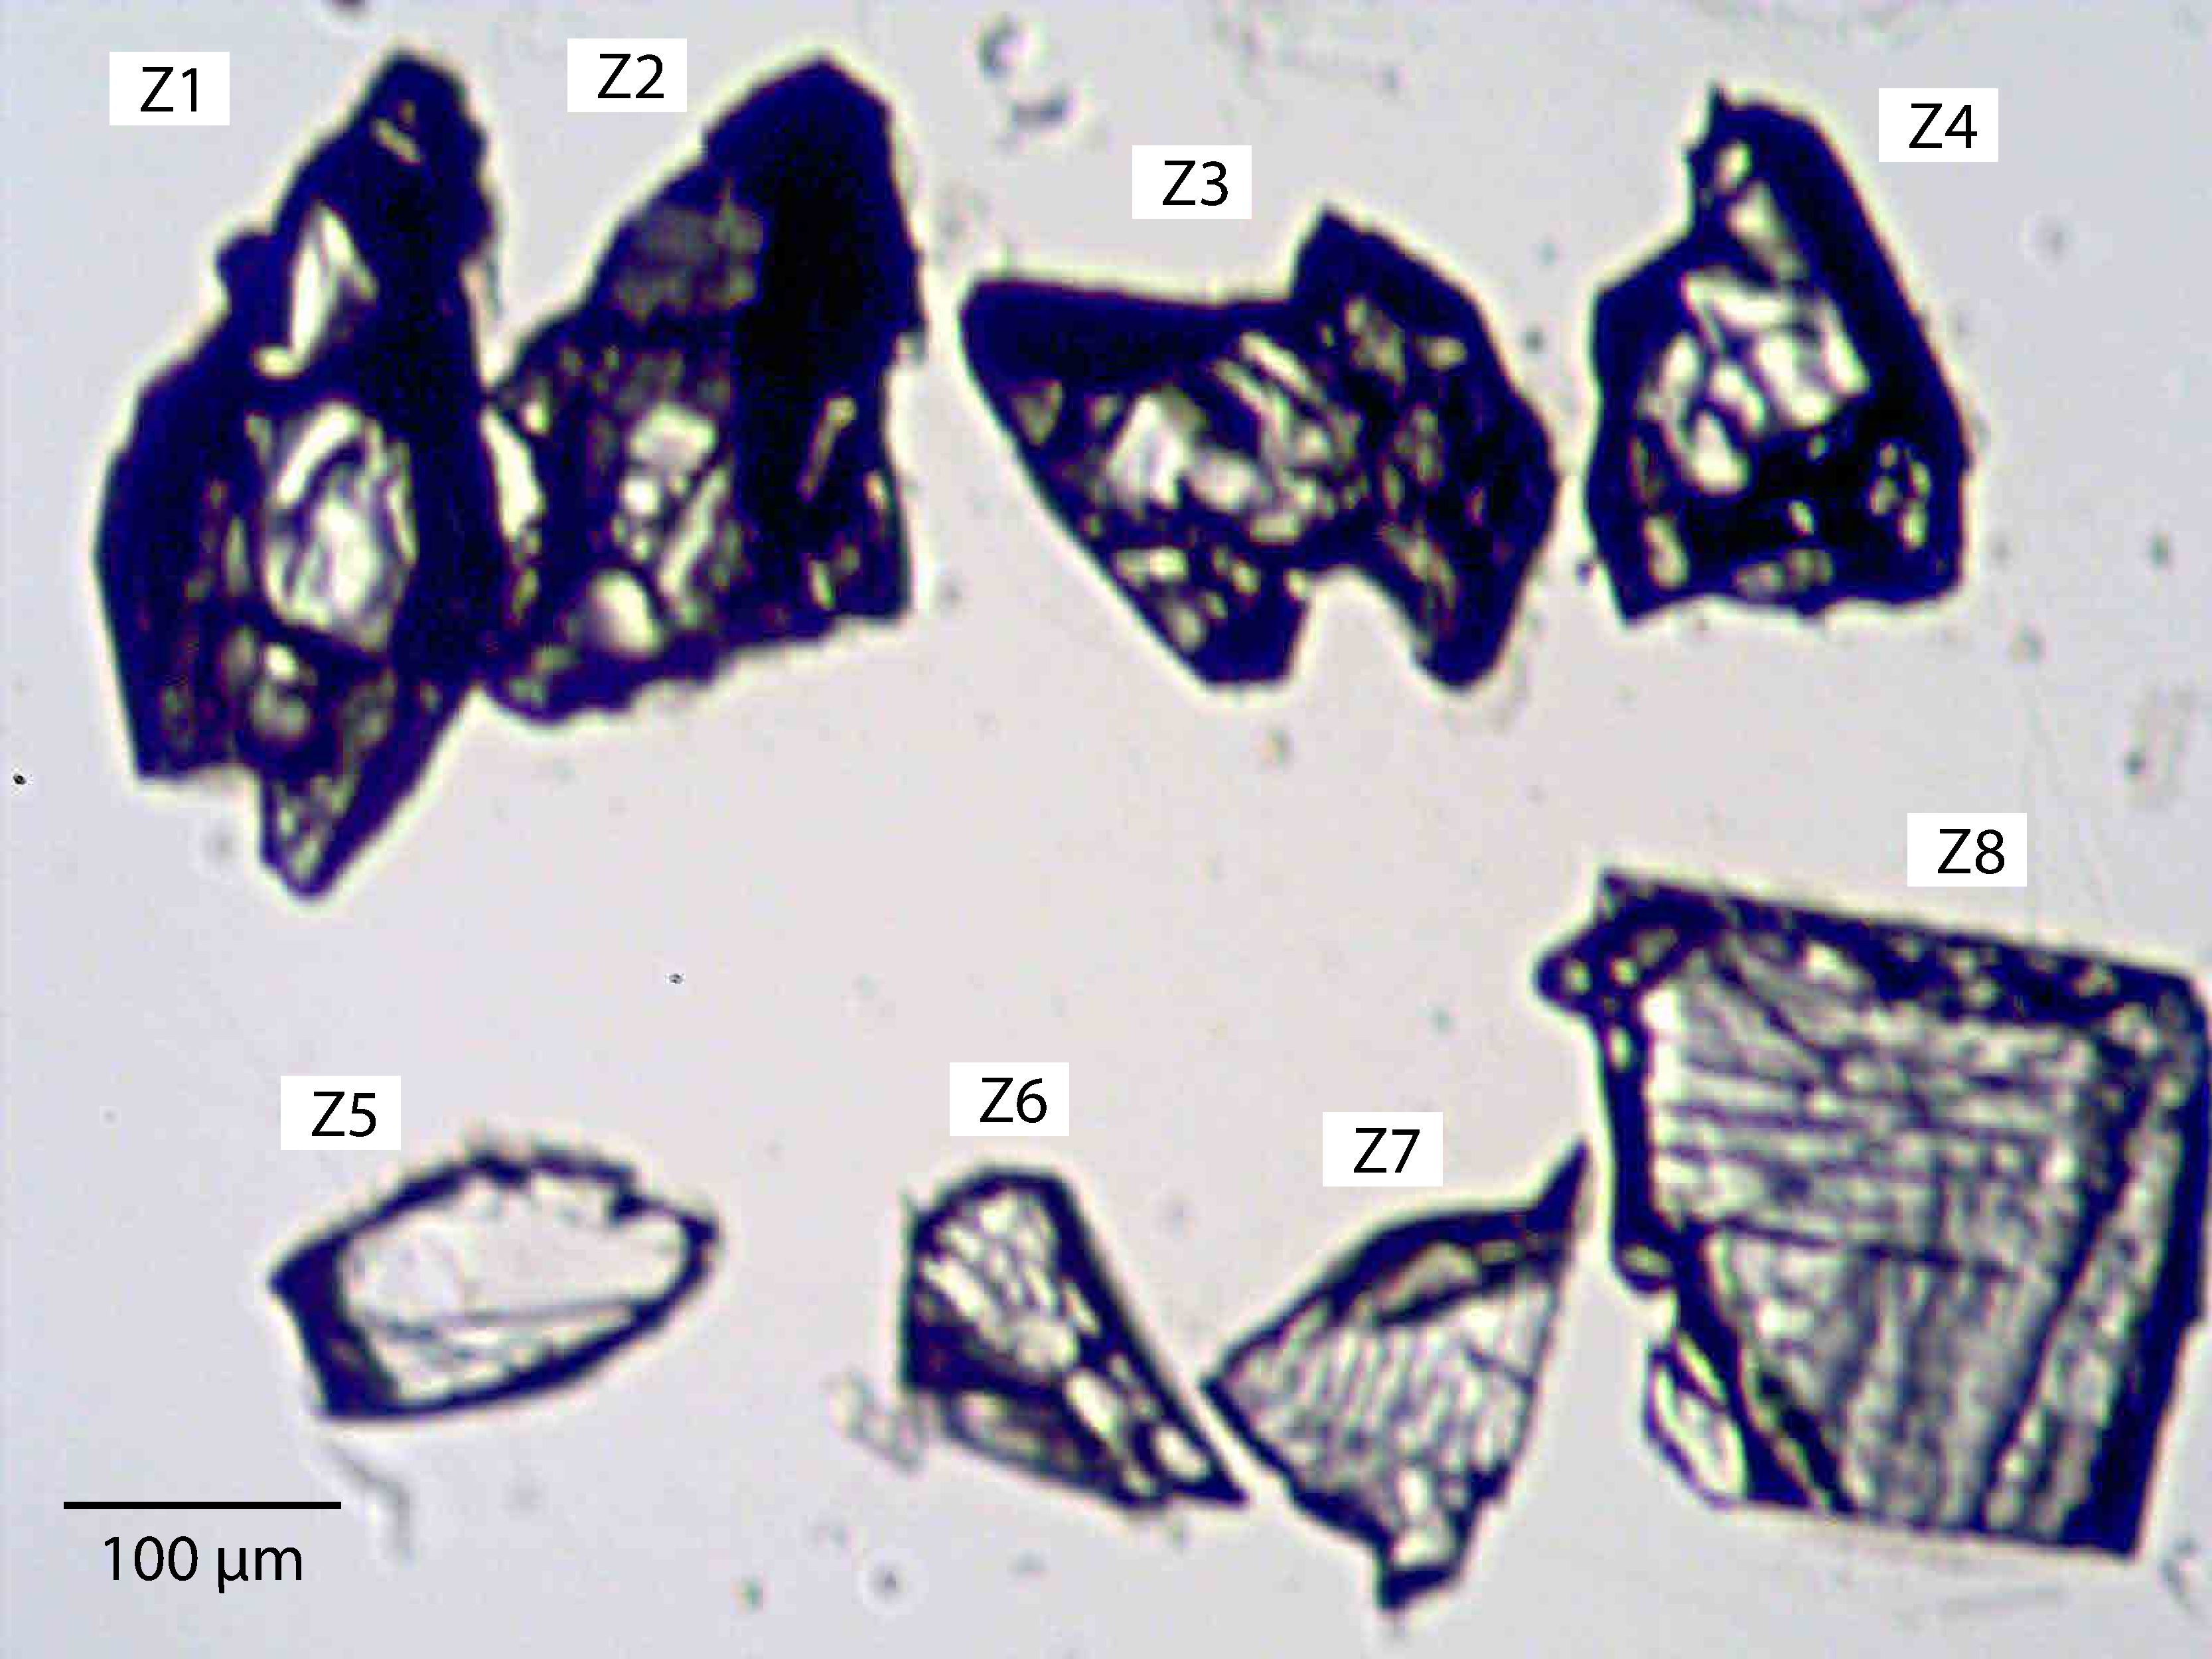
\includegraphics[width=0.9\textwidth]{figure/Zhang2021/SI_zircons.pdf}
\centering
\caption[Image of individual zircons used for ID-TIMS U-Pb geochronology from sample MS99033]{\footnotesize{Image of individual zircons used for ID-TIMS U-Pb geochronology from sample MS99033. Zircons (z1-z4) are subhedral to anhedral crystals and (z5-z8) are platy fragments.}}
\label{fig:zircon_image}
\end{figure}

\begin{figure}[h!]
\noindent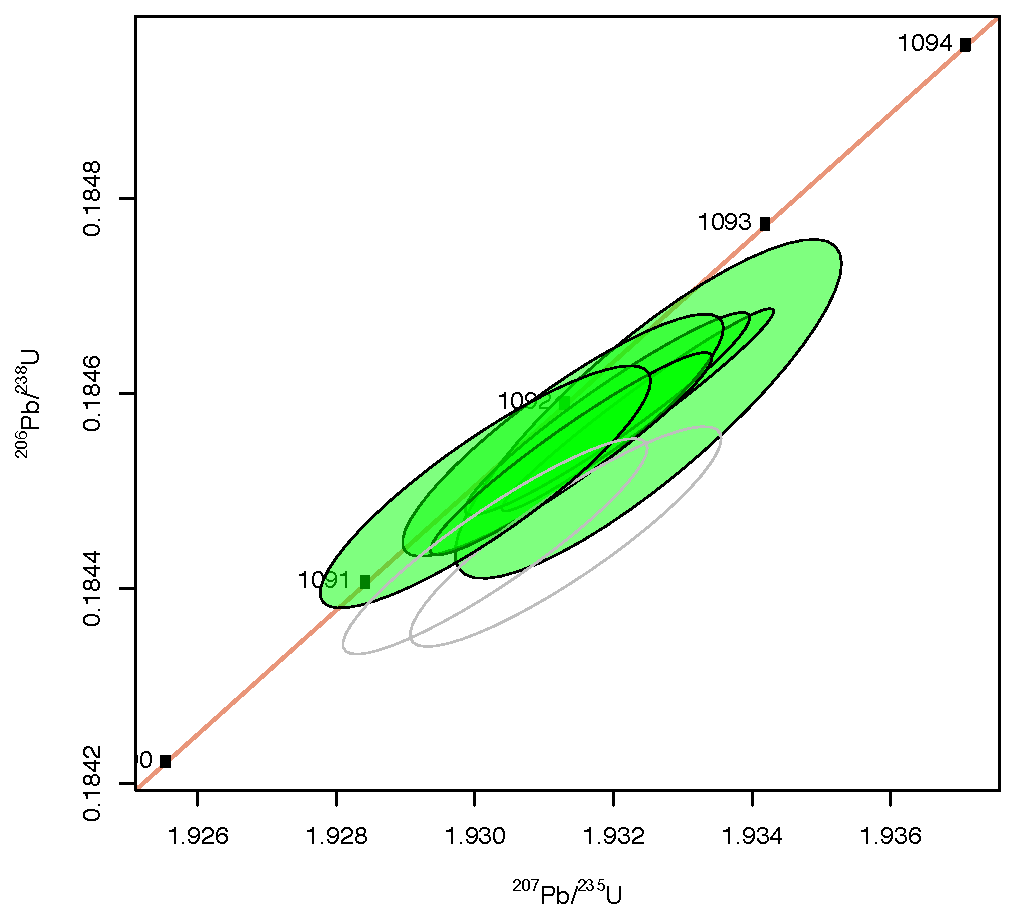
\includegraphics[width=0.8\textwidth]{figure/Zhang2021/SI_MS99033_geochron_plot.pdf}
\centering
\caption[U-Pb concordia plots for the new zircon dates from anorthosite xenoliths AX16, geochronology sample MS99033]{\footnotesize{U-Pb concordia plots for the new zircon dates from anorthosite xenoliths AX16, geochronology sample MS99033. The ellipses represent 2$\sigma$ analytical uncertainty on individual zircon dates. Green filled ellipses are analyses included in the $^{206}$Pb/$^{238}$U weighted mean dates while the grey ellipses are those that were excluded. }}
\label{fig:zircon_concordia}
\end{figure}

U-Pb dates were obtained by chemical abrasion isotope dilution thermal ionization mass spectrometry (ID-TIMS) in the Boise State University (BSU) Isotope Geology Laboratory (Table S2; Fig. \ref{fig:zircon_image}). 

Zircons were separated from the bulk rock sample using a sledge, Retsch DM200 disc mill, 500 µm sieve, Wilfley Shaker Table, LB-1 Frantz magnetic separator, and methylene iodide heavy liquid. Heavy separates were annealed at 900\textdegree C for 48 to 60 hours in quartz crucibles in a muffle furnace. Individual zircons were chemically abraded. Chemical abrasion was carried out by transferring zircons to 3 ml Teflon Perfluoroalkoxy alkane (PFA) beakers in which they were rinsed in 3.5 M HNO$_\mathrm{3}$ and ultrapure H$_\mathrm{2}$O prior to loading into 300 $\mu$l Teflon PFA microcapsules. Fifteen microcapsules were placed in a large-capacity Parr vessel and the zircon partially dissolved in 120 $\mu$l of 29 M HF for 12 hours at 190\textdegree C. Zircons were returned to 3 ml Teflon PFA beakers, HF was removed, and zircons were immersed in 3.5 M HNO$_\mathrm{3}$, ultrasonically cleaned for an hour, and fluxed on a hotplate at 80°C for an hour. The HNO$_\mathrm{3}$ was removed and zircon was rinsed twice in ultrapure H2O before being reloaded into the 300 $\mu$l Teflon PFA microcapsules (rinsed and fluxed in 6 M HCl during sonication and washing of the zircons) and spiked with the $^{233}$U-$^{235}$U-$^{205}$Pb BSU tracer solution (BSU1B). Zircons were dissolved in Parr vessels in 120 $\mu$l of 29 M HF at 220\textdegree C for 48 hours, dried to fluorides, and re-dissolved in 6 M HCl at 180\textdegree C overnight. Pb and U were separated from the zircon matrix using an HCl-based anion-exchange chromatographic procedure \citep{Krogh1973a}, eluted together and dried with 2 $\mu$l of 0.05 N H$_\mathrm{3}$PO$_\mathrm{4}$.

Pb and U were loaded on a single outgassed Re filament in 5 $\mu$l of a silica-gel/phosphoric acid mixture \citep{Gerstenberger1997a}, and Pb and U isotopic measurements made on a GV Isoprobe-T multicollector thermal ionization mass spectrometer equipped with an ion-counting Daly detector. Pb isotopes were measured by peak-jumping all isotopes on the Daly detector for 190 cycles with a mass bias correction of 0.16 $\pm$ 0.03$\%$/a.m.u. (1$\sigma$). Transitory isobaric interferences due to high-molecular weight organics, particularly on $^{204}$Pb and $^{207}$Pb, disappeared within 30-45 cycles, while ionization efficiency averaged 104 cps/pg of each Pb isotope. Linearity (to $\geq$1.4 x 10$^6$ cps) and the associated deadtime correction of the Daly detector were determined by analysis of NBS982. Uranium was analyzed as UO$_2^+$ ions in static Faraday mode on 10$^{12}$ ohm resistors for up to 300 cycles, and corrected for isobaric interference of $^{233}$U$^{18}$O$^{16}$O on $^{235}$U$^{16}$O$^{16}$O with an $^{18}$O/$^{16}$O of 0.00206. Ionization efficiency averaged 20 mV/ng of each U isotope. U mass fractionation was corrected using the $^{233}$U/$^{235}$U ratio of the BSU1B tracer. 

\section*{LA-ICPMS plagioclase geochemistry}

Rare earth elements (REE) ICPMS analyses are done by the GeoAnalytical Lab at Washington State University. Four plagioclase crystals with minimal visible other mineral inclusions from anorthosite sample MS99033 were picked for REE analyses (Table S3). The Flux used for the fusion is di-Lithium-tetraborate (Spectromelt$^@$ A-10, EM Science, Gibbstown, NJ). Reagents are HNO$_3$ 69-70\% (Fisher ACS plus grade), HF 48-52\% (Baker ACS reagent grade), HClO$_4$ 67-71\% (Fisher Trace Metal Grade), and H$_2$O$_2$ (Baker ACS Reagent). The HF is further purified before use by sub-boiling distillation in a Teflon still.  All water used is $>$18 M deionized water from a Nanopure analytical grade water system (Barnstead/Thermolyne)

Powdered samples are mixed with an equal amount of lithium tetraborate flux (typically 2g), placed in a carbon crucible and fused at 1000\textdegree C in a muffle furnace for 30 minutes. After cooling, the resultant fusion bead is briefly ground in a carbon-steel ring mill and a 250 mg portion is weighed into a 30 ml, screw-top Teflon PFA vial for dissolution. The acid dissolution consists of a first evaporation with HNO$_3$ (2ml), HF (6 ml), and HClO$_4$ (2 ml) at 110\textdegree C. After evaporating to dryness, the sample is wetted and the sides of the vial are rinsed with a small amount of water before a second evaporation with HClO$_4$ (2 ml) at 160\textdegree C. After the second evaporation, samples are brought into solution by adding approximately 10 ml of water, 3 ml HNO$_3$, 5 drops H$_2$O$_2$, 2 drops of HF and warmed on a hot plate until a clear solution is obtained. The sample is then transferred to a clean 60 ml HDPE bottle diluted up to a final weight of 60g with deionized water.

Solutions are analyzed on an Agilent model 4500 ICPMS and are diluted an additional 10X at the time of analysis using Agilent’s Integrated Sample Introduction System (ISIS). This yields a final dilution factor of 1:4800 relative to the amount of sample fused. Instrumental drift is corrected using Ru, In, and Re as internal standards. Internal standardization for the REEs uses a linear interpolation between In and Re after \cite{Doherty1989a} to compensate for mass-dependant differences in the rate and degree of instrumental drift. Isobaric interference of light rare earth oxides on the mid- heavy REEs can be a significant source of error in ICPMS analysis, so tuning is optimized to keep the CeO/Ce ratio below 0.5\%. Correction factors used to compensate for the remaining oxide interferences are estimated using two mixed-element solutions. The first contains Ba, Pr, and Nd, and the second Tb, Sm, Eu, and Gd.  Standardization is accomplished by processing duplicates of three in-house rock standards interspersed within each batch of 18 unknowns. Concentrations, oxide- and drift corrections are then calculated offline using a spreadsheet. Methods description is provided by: \url{https://environment.wsu.edu/facilities/geoanalytical-lab/technical-notes/icp-ms-method/}.  


\section*{LA-ICPMS zircon geochemistry}

15 zircons extracted from sample MS99033 were analyzed by laser ablation inductively coupled plasma mass spectrometry (LA-ICPMS) using a ThermoElectron, iCAP-RQ, single quadrupole ICPMS and a Teledyne (Photon Machines) Analyte Excite+ 193 nm excimer Analyte laser with a HelEx ablation cell at BSU. Analytical protocols, standard materials, and data reduction software developed at BSU were used for acquisition and calibration of U-Pb dates and a suite of high field strength elements (HFSE) and rare earth elements (REE). Zircon were ablated with a 25 µm diameter laser spot using fluence and pulse rates of $\sim$2.5 J/cm2 and $\sim$5 Hz, respectively, during a 20-second analysis excavating a pit 25 µm deep. Ablated material was carried to the nebulizer flow of the plasma by a 1.2 L/min He gas stream. Total sweep duration is 895 ms, and quadrupole dwell times were 5 ms for Si and Zr, 40 ms for $^{202}$Hg, $^{204}$Pb, $^{208}$Pb, $^{232}$Th, and $^{238}$U, 80 ms for $^{206}$Pb, 200 ms for $^{49}$Ti and $^{207}$Pb, and 10 ms for all other HFSE and REE. Background count rates were obtained prior to each spot analysis and subtracted from the raw count rate for each analyte. Concentrations were calculated using background-subtracted count rates internally normalized to $^{29}$Si and calibrated with the primary standards NIST SRM-610 and -612 glasses. Ablation pits that intersected mineral inclusions were identified based on Ti and P spikes. The Ti-in-zircon thermometer was calculated using an average TiO$_2$ activity value of 0.7 in crustal rocks \citep{Watson2006a} and an average SiO$_2$ activity value of 1.0 \citep{Ferry2007a}. 

\section*{Additional zircon photomicrograph}
\begin{figure}[h!]
\noindent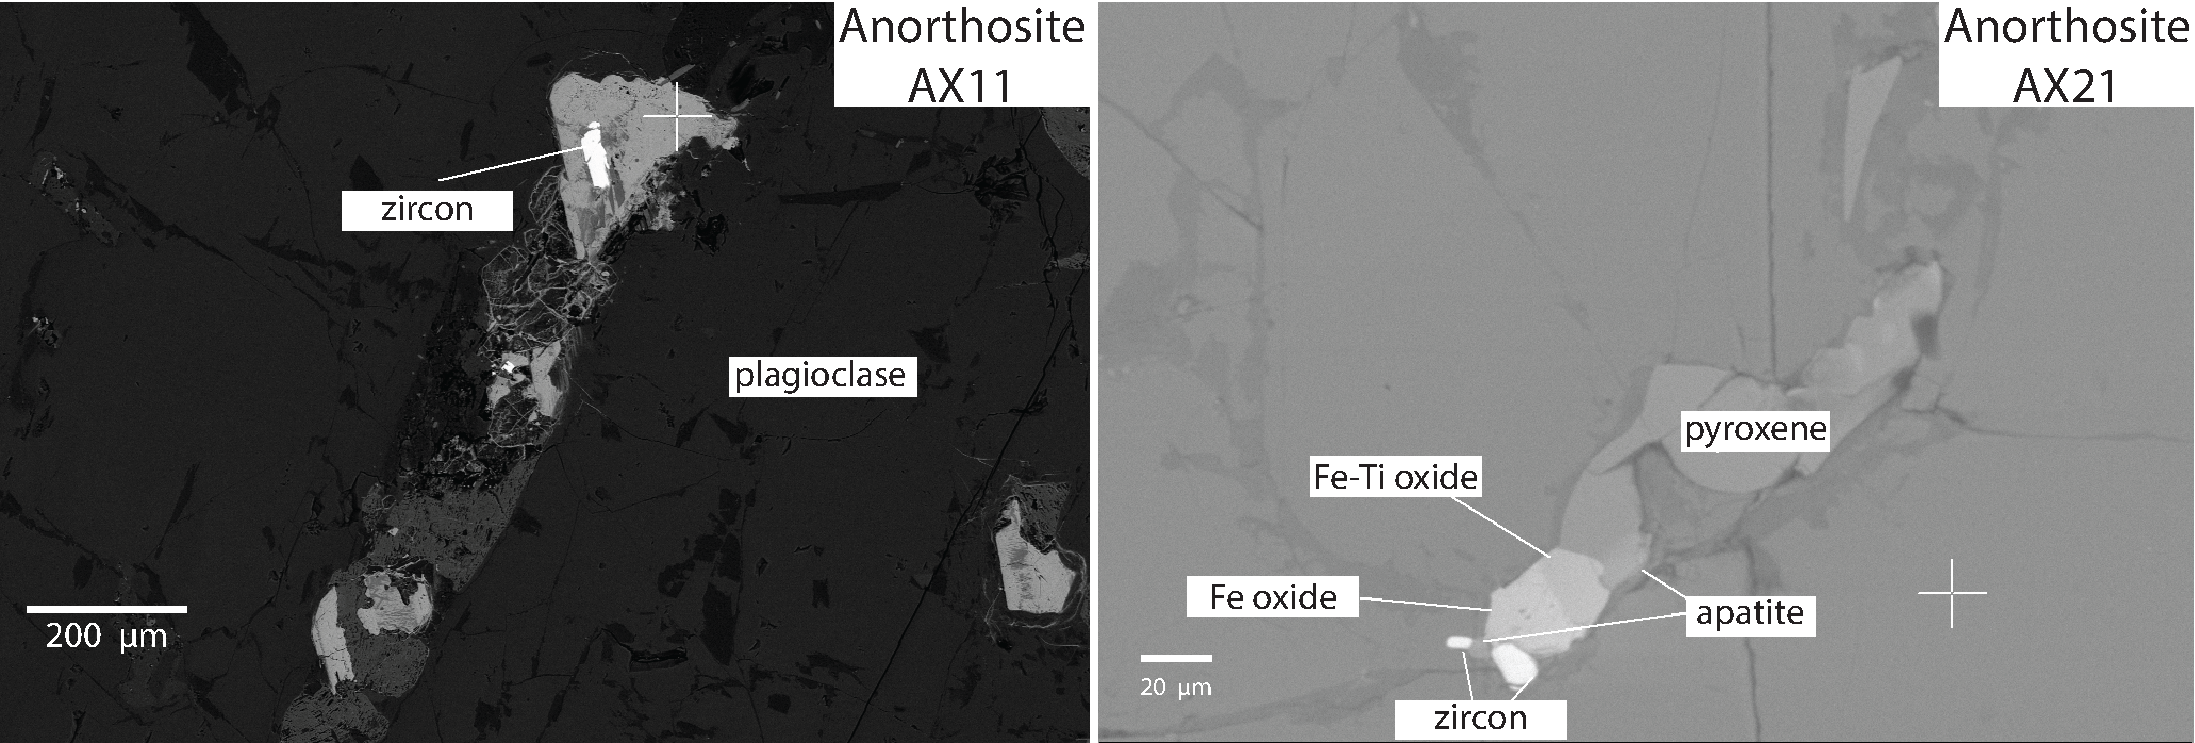
\includegraphics[width=\textwidth]{figure/Zhang2021/SI_interstitial_zircons.pdf}
\caption[Backscattered electron (BSE) images of anorthosite xenoliths.]{\footnotesize{Backscattered electron (BSE) images of anorthosite xenoliths. Subhedral to anhedral zircons form next to mafic melt pockets.}}
\label{fig:interstitial_zircons}
\end{figure}

Fig. \ref{fig:interstitial_zircons} shows subhedral and anhedral zircons in anorthosite xenoliths AX11 and AX21 in back scattered electron (BSE) images of anorthosite thin sections. All zircons found are interstitial to the plagioclase. This texture is consistent with the interpretation of a zircon formation from interstitial melt liquids preserved in plagioclase mush.

\section*{Beaver River diabase structural correction}

Structural measurements were obtained from the published geologic maps of the study area as well as our field data. We calculated the mean directions from the combined volcanic bedding measurements from the Schroeder-Lutsen basalt and igneous layering measurements from the Beaver River diabase and constructed two sets of tilt correction data for the paleomagnetic sites in the southern and eastern Beaver Bay Complex \citep{Boerboom2004a, Boerboom2006a, Boerboom2006b, Boerboom2007a, Miller2001a}. The mean dip angle for the two areas are very similar while the dip trends are different, with the southern Beaver Bay Complex showing a slightly more easterly trend than the eastern Beaver Bay Complex. This difference in dip trend reflects the overall arcuate shape of the Beaver Bay Complex intrusions along the shore of Lake Superior. 

\begin{figure}[h!]
\noindent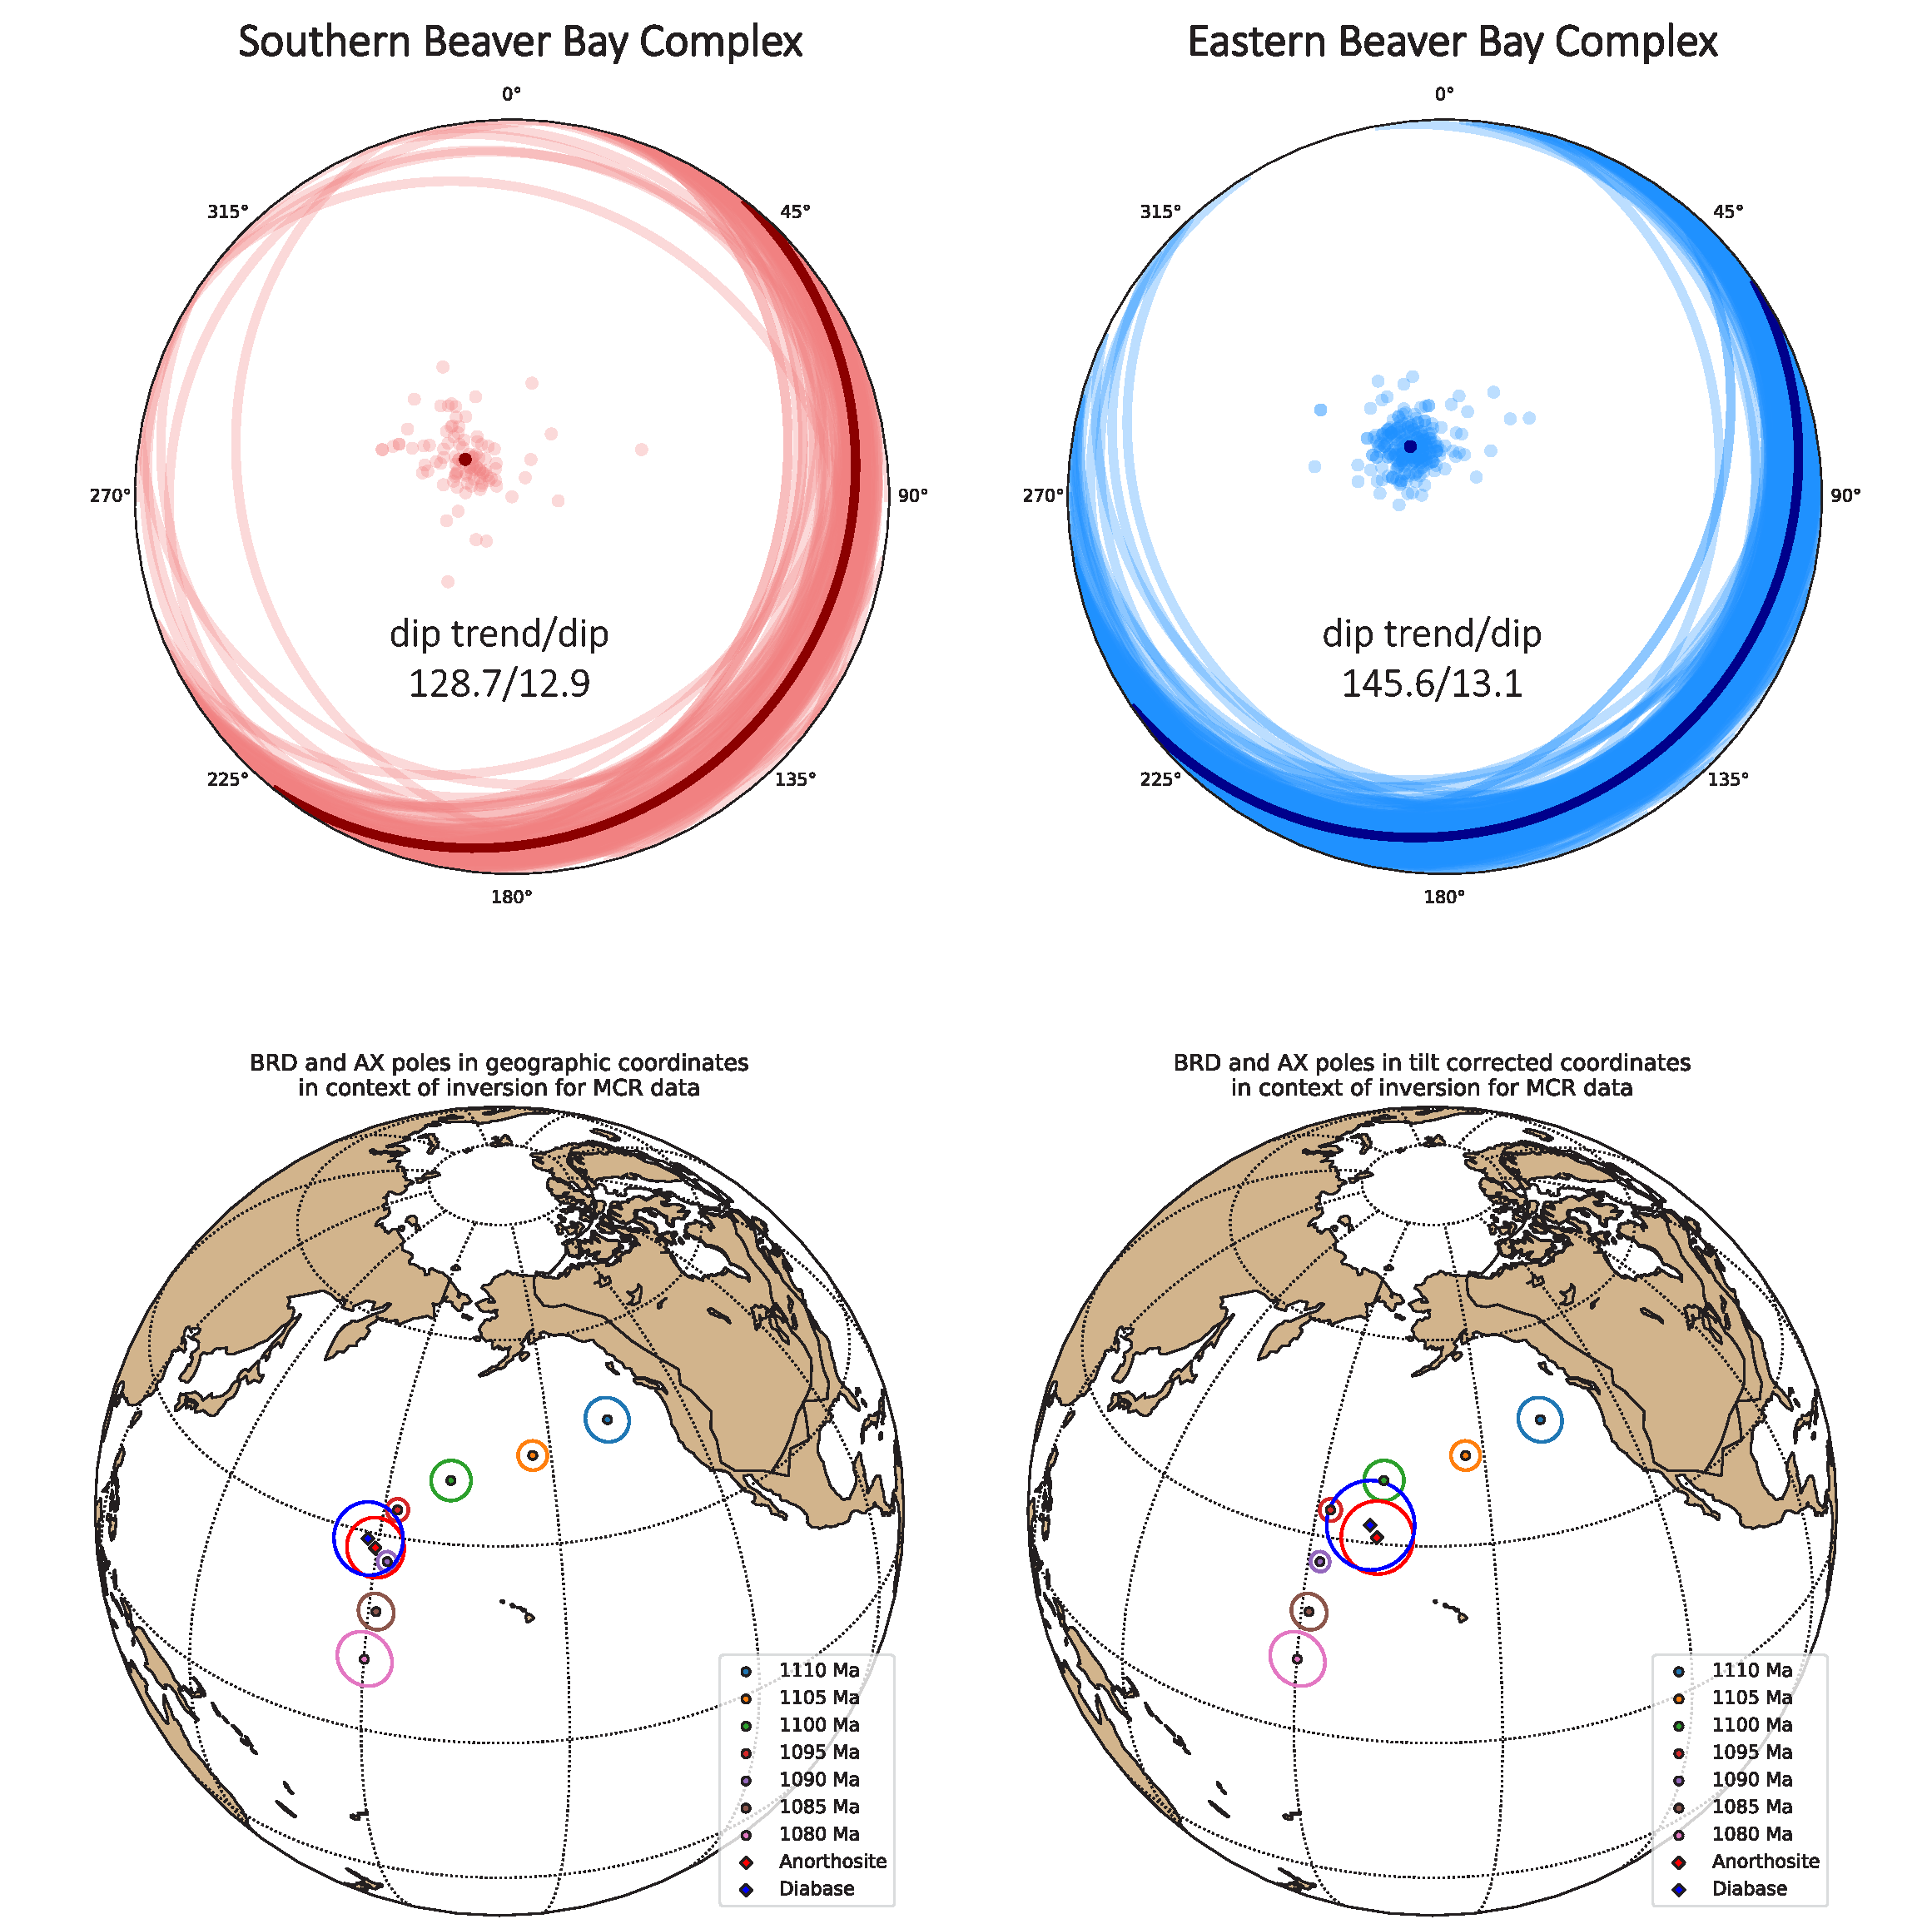
\includegraphics[width=0.9\textwidth]{figure/Zhang2021/SI_tilt_correction.pdf}
\centering
\caption[Tilt correction analyses for the Beaver River diabase and anorthosite paleomagnetic data]{\footnotesize{Stereonet plots of the compiled structural orientation data to tilt correct the paleomagnetic directions obtained from the Beaver River diabase and the anorthosite xenoliths therein. The mean pole position of the diabase and anorthosite units before and after the tilt correction are shown in context of the inverted Keweenawan Track developed by \cite{Swanson-Hysell2019a}.}}
\label{fig:tilt_correction}
\end{figure}

To summarize, We use a bedding dip direction - dip of 145.6 - 13.1 for paleomagnetic site AX3, AX4, AX5, AX6, AX7, AX8, AX9, AX10, and BD2, BD14, BD15, BD16 in the Eastern Beaver Bay Complex region. We use a bedding dip direction - dip of 128.7 - 12.9 for site AX1, AX2, AX11, AX12, AX13, AX14, AX15, AX16, AX17, AX18, AX19, AX20, AX21, AX22, BD1, BD3, BD4, BD5, BD6, BD7. BD8. BD9, BD10, BD11, BD12, BD13, BD17 in the Southern Beaver Bay Complex.

Fig. \ref{fig:tilt_correction} shows the stereonet plots of the bedding orientations compiled for tilt correcting the paleomagnetic directions of samples collected in the Southern Beaver Bay Complex and the Eastern Beaver Bay Complex. The resultant mean pole position for the diabase changes from 29.0\textdegree N, 178.2\textdegree E, N = 15, A95 = 5.2\textdegree, k = 55.3 before tilt correction to 32.5\textdegree N, 189.5\textdegree E, N = 15, A95 = 6.3\textdegree, k = 37.4 after tilt correction. For the anorthosite, the mean pole position changes from 28.0\textdegree N, 179.6\textdegree E, N = 17, A95 = 4.3\textdegree, k = 70.6 before tilt correction to 30.9\textdegree N, 190.8\textdegree E, N = 17, A95: 5.2\textdegree, k = 48.5 after tilt correction. The uncertainty ellipses for both units are slightly larger after tilt correcting the directions. This may reflect the uncertainties associated with using igneous fabrics as our paleohorizontal references. Nevertheless, the mean pole position of the diabase and anorthosite still overlaps and is consistent with the expected position derived from the inverted Keweenawan Track \textit{ca.} 1092 Ma \citep{Swanson-Hysell2019a}. 


\vspace{1in}

\begin{figure}[h!]
\noindent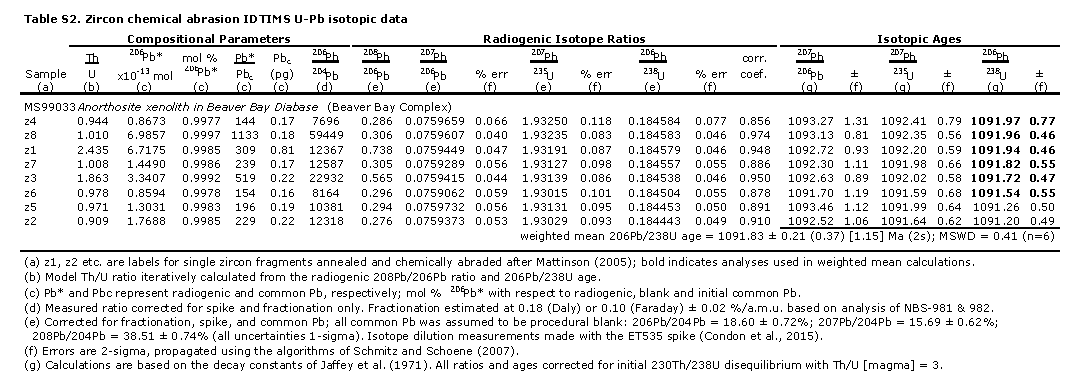
\includegraphics[width=\textwidth]{figure/Zhang2021/SI_MS99033_geochron.pdf}
\centering
\end{figure}

\vspace{1in}

\begin{figure}[h!]
\noindent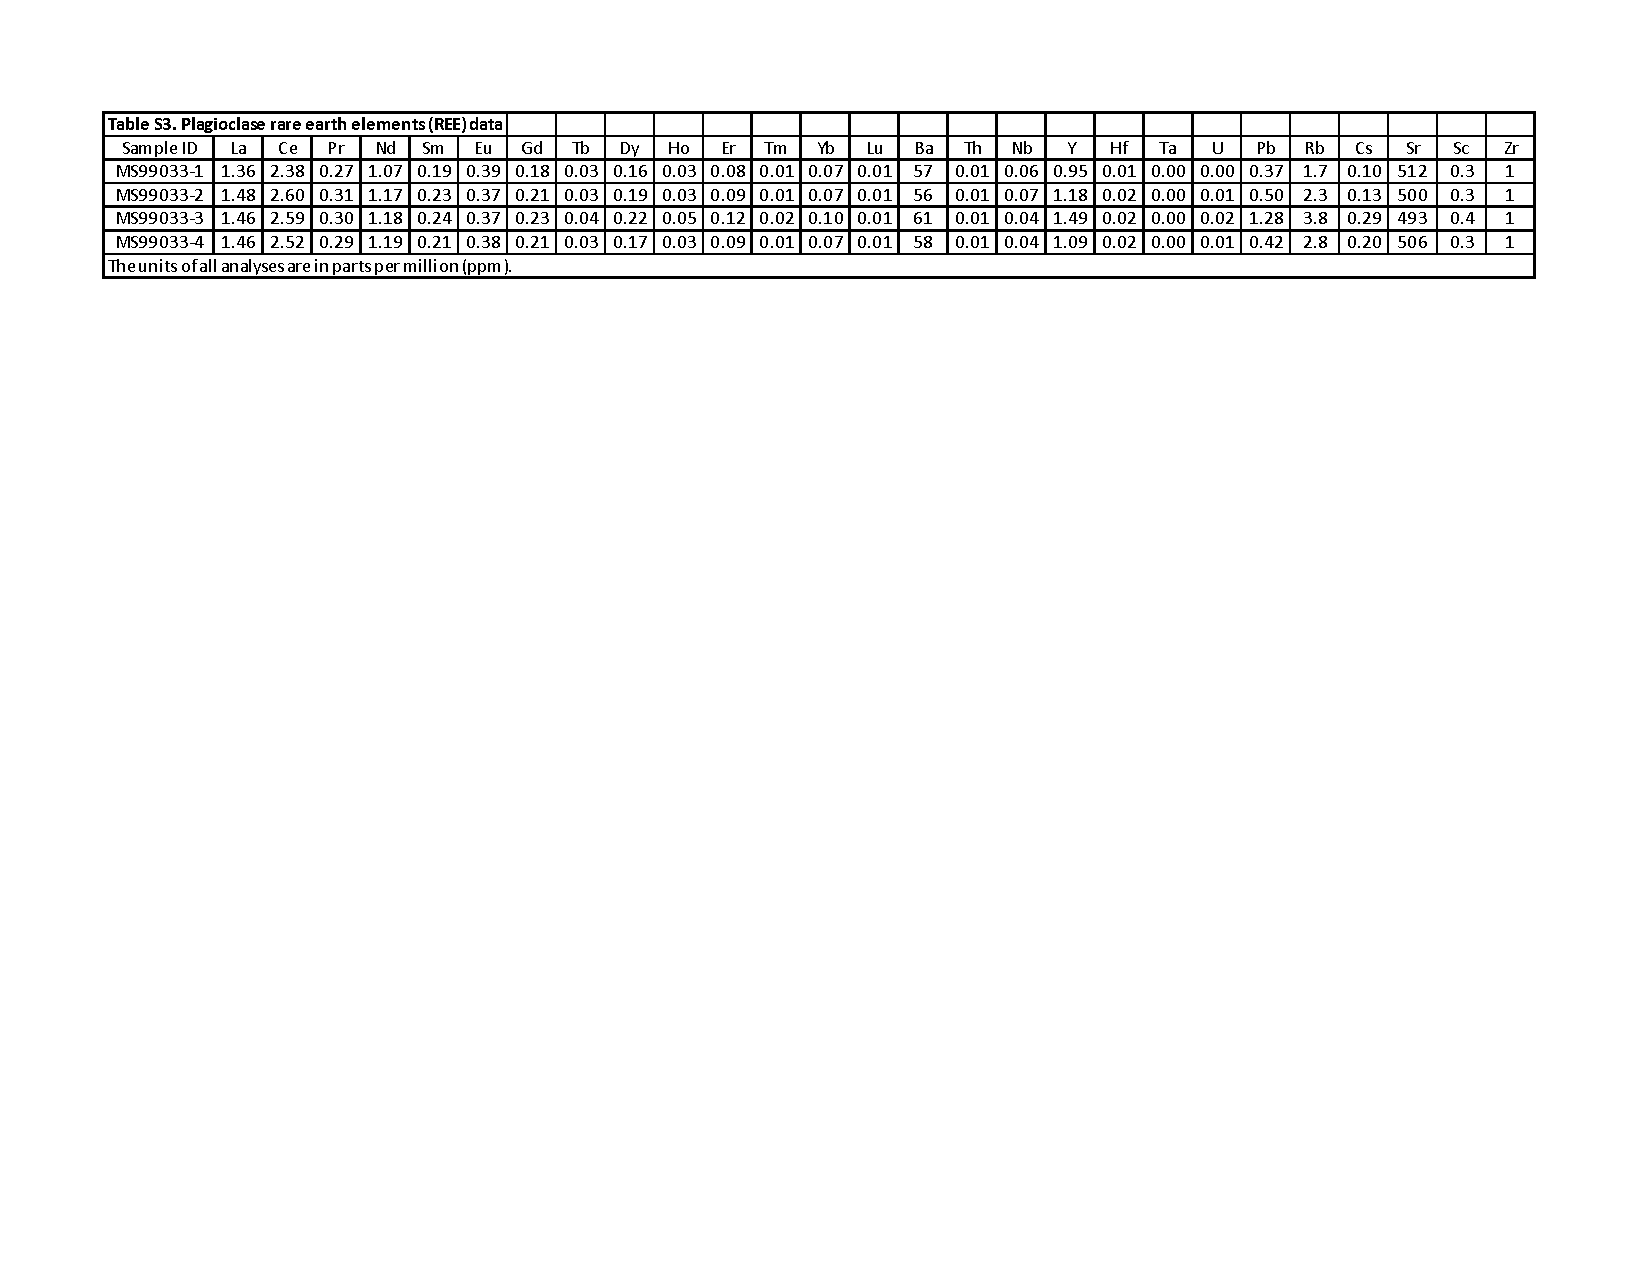
\includegraphics[width=\textwidth]{figure/Zhang2021/SI_plag_REE_table.pdf}
\centering
\end{figure}

\nocite{Mattinson2005a, Condon2015a, Schmitz2007a, Jaffe1975a}

\clearpage

